\section{Methodik}\label{chap:Methodik}

Für die Untersuchung der Auswirkungen der Netzintegration von \glspl{EPKW} auf die Verteilnetze, wird vorerst die Schaffung entsprechende Netztopologien mit Hilfe des Open Source Tools \gls{DINGO} und deren Clusterung beschrieben.
Anschließend werden mit Hilfe des Software Tools \gls{SIMBEV} Fahrtprofile von \glspl{EPKW} erstellt und die untersuchten Ladestrategien beschrieben.
Damit der Ladebedarf in die Netzmodelle integriert werden kann, muss dieser anschließend räumlich auf eine entsprechende georeferenzierte Ladeinfrastruktur verteilt werden.
Abschließend erfolgt eine Beschreibung der Methodik zur Bestimmung von Netzproblemen und der Ermittlung des Abregelungsbedarfs im Netzgebiet mit Hilfe des Open Source Tools \gls{EDISGO}.


\subsection{Erstellung der Verteilnetztopologien}\label{chap:dingo_theo}

Eine der Grundlagen für die Nutzung des Netzplanungsinstruments \glspl{EDISGO}, sind die zu untersuchenden Netztopologien der \gls{MS}- und \gls{NS}-Ebene.
Aufgrund der mangelnden Datenlagen von reale Netztopologien, wird auf synthetisch erzeugte Netztopologien zurückgegriffen, die mit Hilfe des Open Source Tools \gls{DINGO} erzeugt werden.
Das Tool ist in der Lage ländliche und suburbane Netzstrukturen zu synthetisieren und kann auf GitHub \cite{dingo2019} öffentlich eingesehen und frei verwendet werden.
Weiterhin findet sich auf Read the Docs \cite{dingo-docs2019} eine ausführliche Dokumentation.\medskip

Die Synthetisierung der Netztopologien ist nicht Teil dieser Masterarbeit und erfolgte innerhalb des \openego Projektes. \cite{Mueller2019}
Die Netztopologien werden auf der Datengrundlage des Jahres \num{2015} gebildet und entsprechend ausgebaut.
Urbane Netzgebiete können derzeit nicht durch \gls{DINGO} abgebildet werden und werden deshalb innerhalb dieser Masterarbeit nicht betrachtet.


\paragraph{Mittelspannung:}

Die einzelnen \gls{MS}-Netze werden alle als offene Ringnetze betrieben.
Im städtischen Bereich werden hauptsächlich Erdkabel mit einer Nennspannung von \SI{10}{\kv} eingesetzt, während im ländlichen Raum größtenteils Freileitungen mit einer Nennspannung von \SI{20}{\kv} eingesetzt werden. \cite{Mueller2019}\medskip

Die Modellierung der Mittelspannungstopologie erfolgt als Tourenplanungsproblem (\gls{CVRP}) in Kombination mit der Beachtung der historischen lastorientierten Entwicklung und den Planungsprinzipien von Verteilnetzen.
Ein besondere Fokus liegt dabei auf der Beachtung von Leitungsüberlastungen und Verletzungen des Spannungsbandes.
Eine genau Beschreibung der Methodik findet sich in \cite{Amme2018}.


\paragraph{Niederspannung:}

Die \gls{NS}-Ebene wird mit Hilfe von \num{46} Referenznetzsträngen synthetisiert und als Strahlennetze betrieben.
Die Referenznetzsträngen stehen jeweils repräsentativ für eine bestimmte Anzahl an Hausanschlüssen innerhalb einer Netzklasse.
Bei den Netzklassen wird zwischen Land-, Dorf- und Vorstadtnetzen unterschieden
Auf Grundlage der Anzahl an Hausanschlüssen je Ortsnetzstation wird ein Niederspannungsnetz ebenfalls einer Netzklasse zugeordnet.
Die verschiedenen Referenznetzstränge der entsprechenden Netzklasse werden anschließend so miteinander kombiniert, dass für die entsprechende Anzahl an Hausanschlüssen ein typisches Netz generiert wird. \cite{Mueller2019}


\subsection{K-Means-Clustering}

Die große Anzahl an Netzgebieten und die hohe räumliche und zeitliche Auflösung des Netzdatenmodells führen zu inakzeptabel hohen Rechenzeiten.
Um die Komplexität des Modells zu reduzieren, werden mit Hilfe des \kmeans Referenznetzgebiete ausgewählt, die stellvertretend für eine möglichst große Zahl an Netzgebieten stehen.
Das \kmean wurde im Rahmen des \openego Projektes \cite{Mueller2019} entwickelt und wurde innerhalb \cite{Schachler} uverändert angewendet, um \num{15} repräsentative Netzgebiete zu bestimmen.
Innerhalb dieser Arbeit soll eine Teilmenge dieser \num{15} Netzgebiete mit stark unterschiedlichen Charakteristiken untersucht werden.
An dieser Stelle soll das grundlegende Vorgehen erläutert werden. \medskip

Grundlage des \kmeans bildet der \gls{EMA} des Python Paketes \textit{scikit learn}. \cite{scikit-learn2011}
Hierbei kann jedes \gls{MS}-Netz durch die Definition mehrerer numerischer Attribute als Punkt im mehrdimensionalen Raum beschrieben werden.
Der Algorithmus bildet anschließend eine vorgegebene Anzahl \textit{k} an Clustern durch die Minimierung der Summe der quadrierten gewichteten euklidischen Abstände zwischen den originalen Netzknoten und den Clusterzentren.
Für die Bildung der Cluster werden die folgenden vier Attribute verwendet, um die einzelnen \gls{MS}-Netze zu repräsentieren:

\begin{itemize}
	\item Entwicklung der installierten \gls{PV}-Kapazitäten
	\item Entwicklung der installierten Wind-Kapazitäten
	\item Spitzenlast durch \glspl{WP}
	\item Spitzenlast durch \gls{EPKW}
\end{itemize}

Die Regionalisierung der \gls{PV}-, Wind- und \gls{WP}-Kapazitäten erfolgt nach \autoref{chap:Szenariorahmen}.
Da die Simulation aller \gls{EPKW} aufgrund der großen Anzahl nicht für jedes \gls{MS}-Netzgebiet durchgeführt werden kann, muss die Spitzenlast durch \gls{EPKW} bereits im Voraus abgeschätzt werden.
So wird angenommen, dass nach den Hochlaufzahlen des Antriebswende-Szenarios jeder \gls{PKW} durch einen \gls{EPKW} ersetzt wird und jeder \gls{EPKW} im Jahr \SI{12000}{\km} zurücklegt.
Anhand eines durchschnittlichen Verbrauches von \SI{20}{\kwhkm} wird anschließend der Ladebedarf je Gemeinde abgeschätzt.
Anschließend wird der Ladebedarf mit einem beispielhaften Lastprofil auf die Netzgebiete anhand des Flächenanteils der Gemeinde im Netzgebiete verteilt.\medskip

Damit alle Attribute die gleiche Gewichtung erhalten, müssen diese jeweils normiert werden.
In \autoref{eq:norm_attributes} findet sich das entsprechende Vorgehen.

\begin{equation}
	x_{a, i} = \frac{x'_{a, i} - \text{min~} x^{'}_a}{\text{max~} x'_a - \text{min~} x'_a}
	\label{eq:norm_attributes}
\end{equation}

\noindent Wobei:

\addvbuffer[12pt 12pt]{
	\begin{tabular}{>{$}r<{$}@{\ :\ }l}
		x_{a, i} 	& normierter Wert des Attributes $a$ des Netzes $i$  \\
		a	 		& Attribut Index \\
		i			& Netz Index \\
	\end{tabular}
}

\noindent Anschließend durchläuft der Algorithmus folgende Schritte:

\begin{enumerate}
	\item Zufallsinitialisierung von Clusterzentren
	\item E-Step: Die Netzknoten werden dem nächstgelegenen Clusterzentrum zugewiesen
	\item M-Step: Als jeweils neues Clusterzentrum wird der Schwerpunkt der zugewiesenen Netzknoten eines Clusters verwendet
	\item Die Schritte E und M werden so lange wiederholt, bis Konvergenz auftritt
\end{enumerate}


In \autoref{fig:k-means} findet sich eine exemplarische Darstellung des EM-Algorithmus.
In dieser Arbeit wird stellvertretend für das Cluster, dass Netzgebiet mit dem minimalen quadrierten gewichteten euklidischen Abstand zum Clusterzentrum verwendet. \cite{Mueller2019}

\begin{figure}[H]
    \centering
    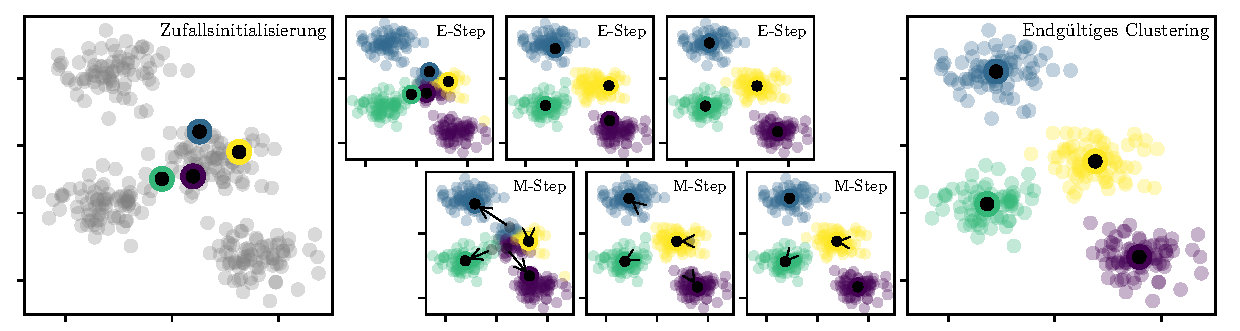
\includegraphics[width=\textwidth]{Bilder/expectation-maximization}
    \caption[Exemplarische Darstellung eines zweidimensionalen Clusterings mit Hilfe des EM-Algorithmus]{Exemplarische Darstellung eines zweidimensionalen Clusterings mit Hilfe des EM-Algorithmus \cite{VanderPlas2016}}\label{fig:k-means}
\end{figure}


\subsection{Erstellung der Fahrtprofile von E-Pkw}\label{chap:simbev_theo}

% TODO: probabilistischen Ansatz mathematisch erklären. @Tim wie wird die Wahrscheinlichkeit je ts konkret festgelegt?

Mit Hilfe des im Rahmen dieser Masterarbeit mitentwickelten Software Tools \gls{SIMBEV} können die Fahrtprofile für eine beliebige Anzahl an Fahrzeugen verschiedener Fahrzeugklassen erstellt werden.
Weiterhin kann hierbei zwischen den in \autoref{tab:RegioStaR} aufgelisteten \glspl{REGIOSTAR} unterschieden werden, um das raumtypenspezifische Fahrverhalten abzubilden.
Zum Zeitpunkt der Erstellung der Fahrtprofile war es noch nicht möglich, einen längeren Zeitraum als eine Woche am Stück zu simulieren.

{
\renewcommand{\arraystretch}{1.2}% grßerer Zeilenabstand
\sisetup{range-phrase=~oder~}
\begin{table}[H]
	\begin{center}
		\caption{Regionalstatistische Raumtypologien 7}
		\begin{tabu} to \textwidth {X[1] X[2]}
			\hline
			Raumtypologie ID	 	& Regionalstatistische Raumtypologie                        \\ \hline
			\num{71}       			& Metropolen                                                \\
			\num{72}       			& Regiopolen und Großstädte                                 \\
			\num{73}       			& Mittelstädte, städtischer Raum einer Stadtregion          \\
			\num{74}       			& Kleinstädtischer dörflicher Raum einer Stadtregion        \\
			\num{75}       			& Zentrale Städte einer Ländlichen Region                   \\
			\num{76}       			& Mittelstädte, städtischer Raum                            \\
			\num{77}       			& Kleinstädtischer, dörflicher Raum einer Ländlichen Region \\ \hline
            \multicolumn{2}{l}{Quelle: \cite{BMVI2020}}
		\end{tabu}
		\label{tab:RegioStaR}
	\end{center}
	\vspace{-3mm}%Put here to reduce too much white space after your table
\end{table}
}

Die Fahrtprofile werden über einen probabilistischen Ansatz auf Grundlage der Befragung \gls{MID} \cite{ISGH2017} erstellt.
Dabei erhält jeder simulierte Zeitschritt eine Wahrscheinlichkeit für einen bestimmten Wegezweck eine Fahrt zu beginnen.
Löst ein Fahrzeug eine Fahrt aus, wird abhängig vom Wegezweck und Regionstyp der Fahrt, ebenfalls probabilistisch, eine Streckenlänge und eine anschließende Standzeit zugeteilt.
Der hierbei entstehende Verbrauch des Fahrzeuges muss anschließend gedeckt werden.
Ob am Zielort ein Ladevorgang stattfindet, hängt vom \gls{SOC} des Fahrzeuges und dem Vorhandensein eines Ladepunktes ab.
Ob ein Ladepunkt am Zielort zur Verfügung steht und welche Ladeleistung dieser aufweist, wird mit Hilfe der Wahrscheinlichkeiten aus \autoref{tab:WegezweckProbability2050} ermittelt.
Ladepunkte besitzen pauschal einen Wirkungsgrad von \SI{90}{\percent}. \cite{EliaGroup2020}
Die Bestimmung des Vorhandenseins eines Ladepunktes zu Hause und am Arbeitsplatz erfolgt je \gls{EPKW} einmalig und wird anschließend konstant gehalten.
Für alle anderen Wegezwecke, erfolgt die Bestimmung kontinuierlich.
Wurde dem Zielort ein Ladepunkt zugeordnet wird davon ausgegangen, dass der Fahrzeugnutzer einen Ladevorgang erst ab einem bestimmten \gls{SOC} einleitet, da dies einen zusätzlichen Aufwand für den Nutzer bedeutet.
Dabei wird angenommen, dass das Laden des Fahrzeuges am Wohnort und am Arbeitsplatz bereits ab einem \gls{SOC} von \SI{95}{\percent} stattfindet.
Im öffentlichen Raum bedeutet das Anfahren und der Anschluss an einen Ladepunkt einen größeren Aufwand für den Nutzer als im privaten Raum.
Deshalb wird angenommen, dass oberhalb eines \glspl{SOC} von \SI{80}{\percent} keine Ladevorgänge stattfinden.
Es gilt je niedriger der \gls{SOC}, desto wahrscheinlicher ist es, dass die öffentliche Ladeinfrastruktur genutzt wird.
Ab einem \gls{SOC} von \SI{50}{\percent} findet, wann immer möglich, eine Ladung des Fahrzeugs statt.
Zwischen den beiden Stützwerten erfolgt eine lineare Interpolation, welche in \autoref{fig:soc_charging_prob} visualisiert wurde.

\begin{figure}[H]
    \centering
    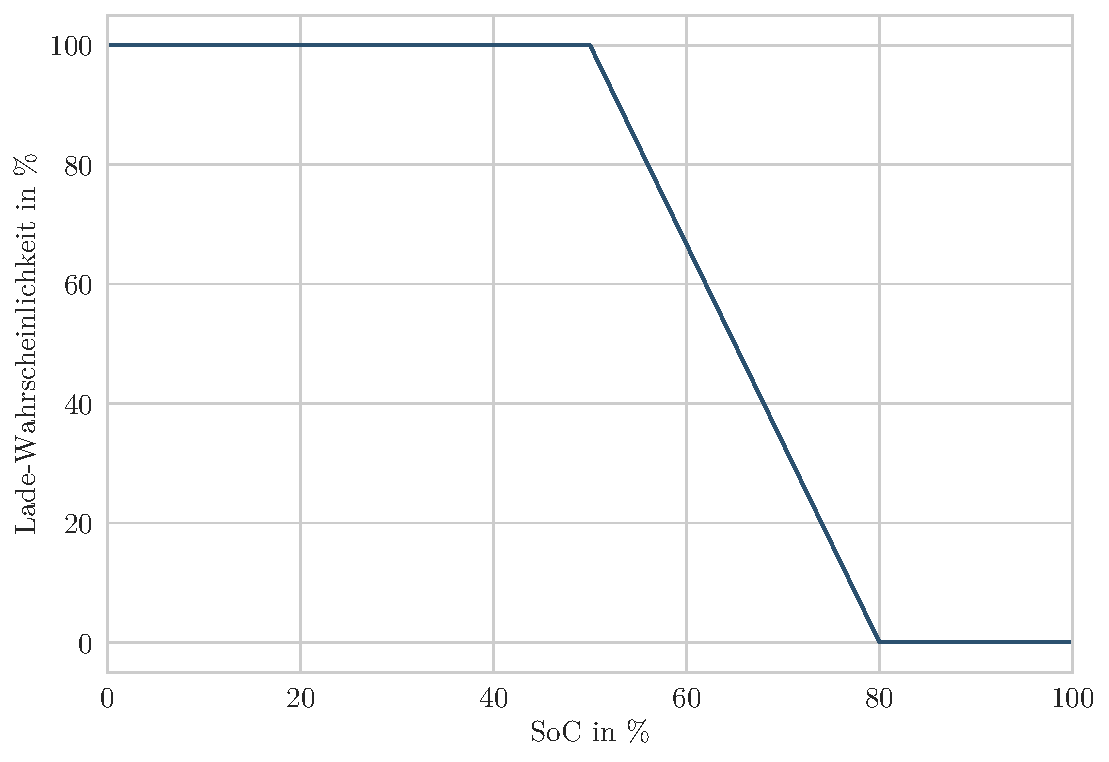
\includegraphics[width=\textwidth]{Bilder/soc_charging_prob}
    \caption{Abhängigkeit der Ladewahrscheinlichkeit vom SoC an öffentlichen Standorten}\label{fig:soc_charging_prob}
\end{figure}

Schnellladeinfrastruktur besitzt aufgrund des zusätzlichen Fahrt- und Zeitaufwandes eine geringe Attraktivität für den Nutzer.
Deshalb wird eine Schnellladung in dieser Simulation nur dann ausgelöst, wenn es wirklich nötig ist.
Sinkt der \gls{SOC} eines Fahrzeugs unter \SI{20}{\percent}, wird eine Schnellladestation angefahren und das Fahrzeug wird für \SI{15}{\Minuten} geladen.
Im Unterschied zu \glspl{BEV}, können \glspl{PHEV} auch mit einem \gls{SOC} von \SI{0}{\percent} ihre Fahrt mit Hilfe des Verbrennungsmotors fortsetzen.
Aus diesem Grund wird bei \glspl{PHEV} kein Schnellladevorgang ausgelöst.\medskip

Um die Anzahl an Fahrzeugen je Netzgebiet zu bestimmen, muss der Gesamtbestand an Fahrzeugen je Szenario (s. \autoref{tab:SzenarienRampUp} und \autoref{tab:CarSplit}) regionalisiert werden.
Die Regionalisierung der Fahrzeuge findet vorerst auf Ebene der Landkreise statt.
Als Grundlage hierfür dient der aktuelle Fahrzeugbestand nach Zulassungsbezirken \cite[][Stand: \DTMdate{2020-01-01}]{KBAPLZ2020}.
Es wird davon ausgegangen, dass es zu keiner Verschiebung des Anteils am Bestand zwischen den Zulassungsbezirken kommt.
Dies bedeutet, dass die Gesamtanzahl der Fahrzeuge je Fahrzeugklasse je Szenario entsprechend des heutigen Bestandes anteilig verteilt wird.
Die Aufteilung der Fahrzeuge in Klassen erfolgt anhand der Einteilung des Fahrzeugsbestands in Hubraum-Klassen, welche ebenfalls dem Fahrzeugbestand nach Zulassungsbezirken entnommen werden können.\medskip

Die geographische Einteilung der Landfläche in \glspl{REGIOSTAR} erfolgt auf Gemeindeebene, weshalb eine weitere Regionalisierung der Fahrzeuge innerhalb eines Landkreises auf die jeweiligen Gemeinden nötig ist.
Da auf Gemeindeebene keine Daten zum Fahrzeugbestand vorliegen, erfolgt die Regionalisierung anhand der Einwohnerzahl der Gemeinden.
Die Grundlage hierfür bildet der Datensatz \glqq Gemeindegrenzen 2017 mit Einwohnerzahl\grqq{} \cite[][Stand: \DTMdate{2017-12-31}]{EDG2020}.
Die Verteilung der Anzahl der Fahrzeuge erfolgt streng proportional zur Einwohnerzahl in der jeweiligen Gemeinde.
Jedes \gls{MS}-Netzgebiet streckt sich dabei in der Regel über mehrere Gemeinden, wobei einzelne Gemeinden auch nur anteilig innerhalb eines Netzgebietes liegen können.\medskip

Um abschließend die Fahrtprofile erzeugen zu können, muss jeder Gemeinde eine \gls{REGIOSTAR} Nummer zugeordnet werden.
Die entsprechende Zuordnung für das Jahr \num{2018} kann dem Datensatz \glqq Referenzdateien zur regionalstatistischen Raumtypologie\grqq{} \cite[][Stand: \DTMdate{2018-01-01}]{BMVIa2020} entnommen werden.


\subsection{Räumliche Verteilung der Ladevorgänge}\label{chap:theo_distribution}

Die räumliche Verteilung der Ladevorgänge innerhalb eines geographischen Gebietes kann starken Einfluss auf die Auswirkungen der Netzintegration von \glspl{EPKW} haben.
So können beispielsweise regionale Konzentration von Ladepunkten einzelne Leitungen stark beanspruchen und den Netzausbaubedarf erhöhen.\medskip

Innerhalb dieser Arbeit erfolgt die Verteilung der Ladevorgänge immer innerhalb des untersuchten geographischen Gebietes.
Ein Laden in anderen geographischen Gebieten, oder das Laden von \glqq Fremdfahrzeugen\grqq{} im untersuchten Gebiet kann nicht abgebildet werden.
Grundlage für die Ermittlung von möglichen Standorten bietet eine geoinformatische Auswertung der untersuchten geographischen Gebiete.
Das hierfür verwendete Software Tool, wurde unabhängig von dieser Arbeit am Reiner Lemoine Institut entwickelt und wurde noch nicht veröffentlicht.
An dieser Stelle soll die Methodik für die Ermittlung von möglichen Standorten und deren Gewichtung für private und öffentliche Ladeinfrastruktur erläutert werden.
Eine genauere Beschreibung der Unterteilung in private und öffentliche Ladeinfrastruktur findet sich in \autoref{chap:EMob_Szenarien}.


\paragraph{Private Ladeinfrastruktur:}

Die private Ladeinfrastruktur beinhaltet alle Ladevorgänge, die an privater Ladeinfrastruktur am Eigenheim, in Wohnanlagen oder am Arbeitsplatz stattfinden.
Um mögliche Standorte für die Ladeinfrastruktur am Eigenheim oder in Wohnanlagen identifizieren zu können, werden die Anzahl an Wohneinheiten auf einem \SI{100 x 100}{\m} Raster aus dem Zensus 2011 \cite{StatistischesBundesamt2011} verwendet.
So wird jedem Raster mit mehr als einer Wohneinheit und einer Einwohnerzahl von größer Null ein möglicher Anschlusspunkt für Ladeinfrastruktur zugeordnet und anhand der Gesamtanzahl von Wohneinheiten im Raster gewichtet.\medskip

Für private Ladeinfrastruktur am Arbeitsplatz werden die Klassifizierungen der Landflächen nach Nutzungsart nach der \gls{OSM} \cite{OpenStreetMapFoundation} verwendet.
Hierbei wird jeder Landfläche mit der Nutzungsart \glqq commercial\grqq , \glqq retail\grqq{} oder \glqq industrial\grqq{} ein möglicher Anschlusspunkt für Ladeinfrastruktur zugeordnet.
Die Gewichtung erfolgt anhand der Fläche des Gebietes multipliziert mit einem Flächnutzungsfaktor.
Der Flächennutzungsfaktor liegt für \glqq commercial\grqq{} bei \num{3}, für \glqq retail\grqq{} bei \num{2} und für \glqq industrial\grqq{} bei \num{1}.
Da hierdurch unter Umständen nur wenige Anschlusspunkte generiert werden, werden ergänzend \SI{30}{\percent} der möglichen öffentlichen Normalladeinfrastruktur zusätzlich für Ladeinfrastruktur am Arbeitsplatz genutzt.
Den zusätzlichen Anschlusspunkten wird eine geringe Gewichtung zugeordnet, da durch diese vor allem kleine Betriebe abgebildet werden sollen.


\paragraph{Öffentliche Ladeinfrastruktur:}

Die öffentliche Ladeinfrastruktur beinhaltet Ladeinfrastruktur, die nicht der privaten Ladeinfrastruktur zugeordnet werden kann.
Grundsätzlich lässt sich hierbei zwischen Normal- und Schnellladeinfrastruktur unterscheiden.
Für die Normalladeinfrastruktur werden allen \glspl{POI} aus der \gls{OSM} \cite{OpenStreetMapFoundation} in dem untersuchten Gebiet jeweils ein möglicher Anschlusspunkt für Ladeinfrastruktur zugeordnet.
Die Gewichtung der Anschlusspunkt erfolgt hierbei anhand der Gesamtanzahl an \glspl{POI} in der Nähe des Anschlusspunktes.\medskip

Für Schnellladeinfrastruktur werden jeder Tankstelle aus der \gls{OSM} \cite{OpenStreetMapFoundation} im untersuchten Gebiet jeweils ein Anschlusspunkt zugeordnet.
Liegt innerhalb des Gebietes keine Tankstelle, so wird ein zufälliger Anschlusspunkt der öffentlichen Ladeinfrastruktur verwendet.
Eine Gewichtung findet in diesem Fall nicht statt.


\paragraph{Zuteilung der Ladevorgänge auf die Ladeinfrastruktur:}

Die Zuteilung der Ladevorgänge auf die Ladeinfrastruktur erfolgt mit Hilfe des Gewichtungsfaktors der verschiedenen Anschlusspunkte.
Mit Hilfe des Zufallsmoduls des Open Source Tools \textit{NumPy} \cite{harris2020array}, erfolgt eine zufällige und gewichtete Auswahl eines Anschlusspunktes je Ladevorgang.
Im Falle der privaten Ladeinfrastruktur wird für jedes Fahrzeug ein eigener Ladepunkt eingerichtet.
Diesem Ladepunkt werden alle Ladevorgänge des jeweiligen Fahrzeuges und \UCs zugeordnet.
Nachdem einem Anschlusspunkt ein Ladepunkt zugeordnet wurde, wird die Gewichtung des Anschlusspunktes leicht abgesenkt.\medskip

Für die öffentliche Ladeinfrastruktur erfolgt die Zuweisung dezidiert pro Ladevorgang.
So wird je Ladevorgang untersucht, ob bereits ein passender Ladepunkt zur Verfügung steht.
Hierbei wird beachtet, ob in dem entsprechenden Zeitraum der Ladepunkt durch ein anderes Fahrzeug besetzt ist und ob der Ladepunkt die entsprechende Ladeleistung zur Verfügung stellen kann.
Sollte kein passender Ladepunkt zur Verfügung stehen, wird analog zum Vorgehen bei der privaten Ladeinfrastruktur ein Ladepunkt zufällig und gewichtet ausgewählt und eingerichtet.\medskip

Da die \gls{MS}-Netzgebiete nicht immer die Gesamtfläche einer Gemeinde abdecken, muss abschließend geprüft werden, ob die generierten Anschlusspunkte innerhalb des Netzgebietes liegen.
Liegt ein Anschlusspunkt innerhalb eines \gls{MS}-Netzgebietes, so wird er diesem zugeordnet.
Tut dieser es nicht, dann entfällt die Ladevorgänge auf ein angrenzendes Netzgebiet und ist somit nicht Teil der abschließenden Auswertungen.


\subsection{Ladestrategien}\label{chap:theo_strategies}

Innerhalb dieser Arbeit werden zwei präventive Ladestrategien und eine kurative Ladestrategie untersucht.
Das Ziel der Ladestrategien ist es, ein möglichst netzfreundliches Verhalten der Ladevorgänge zu erzeugen, ohne den Nutzen des Fahrzeuges für den Endverbraucher einzuschränken.
Deshalb gilt als Randbedingung aller Ladestrategien, dass der Ladebedarf jedes Ladevorgangs zu \SI{100}{\percent} gedeckt werden muss.
Dies bedeutet, dass Ladevorgänge nur dann flexibilisiert werden können, wenn innerhalb der Standzeit eine Vollladung des Fahrzeuges möglich ist.
Weiterhin können nur private Ladevorgänge flexibilisiert werden, da bei öffentlichen Ladevorgängen die Erfüllung der Dienstleistung im Vordergrund steht.\medskip

Um die drei Ladestrategien miteinander vergleichen zu können, wird zusätzlich ein vollkommen ungesteuertes Laden der Fahrzeuge untersucht, welches als Vergleichspunkt verwendet wird.
Auf diese Weise soll untersucht werden, inwieweit eine kurative Ladestrategie gegenüber präventiven Ladestrategien Vorteile aufweist.
Dies ist deshalb von Bedeutung, da für kurative Eingriffe zusätzliche Technik eingesetzt und die  Betriebsführung dieser abgebildet werden muss, wodurch die Kosten einer kurative Ladestrategie deutlich über den Kosten einer präventiven Ladestrategie liegen.


\paragraph{Gruppiertes Laden:}

Das Ziel des gruppierten Ladens ist es, die Netzbelastung durch die Senkung der Gleichzeitigkeit der Ladevorgänge zu reduzieren.
Hierfür werden die einzelnen Ladepunkte in zwei Gruppen eingeteilt.
Beiden Gruppen werden alternierend 15-minütige Ladezeitfenster zugewiesen, in denen bei voller Ladeleistung der Ladebedarf gedeckt wird.
Es wird darauf geachtet, dass die Zuweisung der Gruppen nicht nur innerhalb eines Netzgebietes ausgeglichen erfolgt, sondern detailliert bis in die einzelnen Stränge der \gls{NS}-Ebene.
Innerhalb eines \gls{NS}-Stranges wird weiterhin darauf geachtet, dass auch die einzelnen Leistungsklassen der Ladeinfrastruktur gleichmäßig auf die Gruppen verteilt werden.
In \autoref{fig:group_vis} findet sich eine beispielhafte Einteilung von Ladepunkten auf die zwei Gruppen innerhalb eines \gls{NS}-Stranges.

\begin{figure}[H]
    \centering
    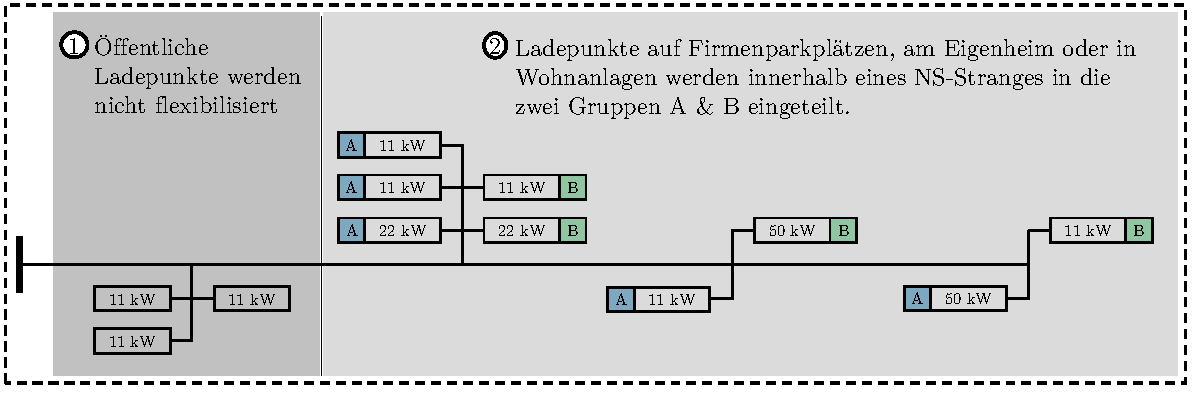
\includegraphics[width=\textwidth]{Bilder/grouped_charging_vis_cropped}
    \caption{Einteilung der Ladepunkte eines NS-Stranges in die Gruppen A \& B für das gruppierte Laden}\label{fig:group_vis}
\end{figure}


\paragraph{Reduziertes Laden:}

Im Gegensatz zum gruppierten Laden soll beim reduzierten Laden die Senkung der Netzbelastung durch die Reduzierung der Ladeleistung der einzelnen Ladevorgänge erreicht werden.
Hierbei wird durch eine Absenkung der Ladeleistung möglichst die gesamte Standzeit des Fahrzeuges für den Ladevorgang ausgenutzt.
Die Flexibilität dieser Ladestrategie wird durch eine Mindestladeleistung von \SI{10}{\percent} der Nennleistung des angefahrenen Ladepunktes technisch begrenzt.

% TODO: Quelle Konferenzpaper Birgit?


\paragraph{Residuallast-Laden:}

Bei dem Residuallast-Laden handelt es sich um eine kurative Ladestrategie.
Der Ladevorgang eines Fahrzeuges findet hierbei immer innerhalb der Zeitpunkte der Standzeit statt, welche die geringste Residuallast innerhalb des Netzgebietes aufweisen, wodurch eine Glättung der Residuallast erreicht werden soll.
Die Zuweisung findet auf Viertelstundenbasis statt und die Ladevorgänge finden immer bei voller Ladeleistung statt.
Das Ziel der Optimierung kann nach \autoref{eq:residual} so formuliert werden, dass eine Minimierung der \gls{MQA} der Residuallast vom Mittelwert der Residuallast angestrebt wird.

\begin{equation}
	\text{MQA} = \frac{1}{n} \sum_i^n \left( P_{\text{R}_i} - \overline{P}_{\text{R}} \right)^2 \stackrel{!}{=} \text{min}
	\label{eq:residual}
\end{equation}

\noindent Wobei:

\addvbuffer[12pt 12pt]{
	\begin{tabular}{>{$}r<{$}@{\ :\ }l}
		P_{\text{R}_i}				& Residuallast zum Zeitschritt $i$  \\
		\overline{P}_{\text{R}}		& Mittelwert der Residuallast 		\\
		n							& Anzahl an Zeitschritten			\\
		i							& Index des Zeitschrittes 			\\
	\end{tabular}
}

Durch die Abhängigkeit der Residuallast von den einzelnen Ladevorgängen sind auch die Ergebnisse der Optimierung der einzelnen Ladevorgänge voneinander Abhängig.
Hierdurch entsteht ein komplexes Optimierungsproblem.
Um die Rechenzeit in einem akzeptablen Maß zu halten, wird eine Näherung an eine optimale Lösung angestrebt.
So wird für jeden Ladevorgang ermittelt, wie viel überschüssige Standzeit zur Flexibilisierung der Ladevorgänge zur Verfügung steht.
Die Ladevorgänge werden anschließend in Abhängigkeit dieses Kriteriums in aufsteigender Reihenfolge sortiert und einzeln optimiert.
Auf diese Weise werden Ladevorgänge mit einem geringen Flexibilitätsband vorrangig behandelt und eine möglichst optimale Lösung bei einem geringen Rechenaufwand erreicht.


\subsection{Netzuntersuchung}\label{chap:edisgo_theo}

Das Open Source Tool \gls{EDISGO} stellt eine Toolbox zur Verfügung, um Verteilnetze auf Netzprobleme zu untersuchen.
Gleichzeitig können mit \gls{EDISGO} Maßnahmen zur Behebung der Netzprobleme bewertet werden.
Dabei bilden synthetische Netztopologien, die mit Hilfe des Open Source Tools \gls{DINGO} erzeugt wurden, die Grundlage für die Berechnungen mit \gls{EDISGO}.
\gls{EDISGO} kann über GitHub \cite{edisgoGit2019} abgerufen werden und ist auf Read the Docs \cite{edisgoDocs2017} dokumentiert.
Innerhalb dieses Kapitels werden die wichtigsten Funktionalitäten \glspl{EDISGO} für die Durchführung der Berechnungen innerhalb dieser Masterarbeit dargestellt und erläutert.


\paragraph{Ermittlung von Netzproblemen:}\label{chap:grid_issues}

Die Überprüfung der einzelnen Netze auf Netzprobleme erfolgt in zwei Schritten.
Vorerst wird eine nichtlineare Lastflussberechnung durchgeführt, um anschließend die Einhaltung der Spannungsanforderungen und technischen Richtlinien bezüglich der Gerätebelastungen zu überprüfen.
Die Durchführung der Lastflussberechnung erfolgt mit Hilfe des Open Source Tools \textit{PyPSA} \cite{Brown2020}.
In diesem Kapitel soll auf die theoretischen Grundlagen der Lastflussberechnung, den Umfang der Analyse und die Spannungsanforderungen und technischen Richtlinien bezüglich der Gerätebelastungen eingegangen werden.\medskip

Das Ziel der Lastflussberechnung ist es, das für jeden Netzknoten $i$ und etwaige Querleitwerte $j$ die folgende Gleichung erfüllt wird:

\begin{equation}
	S_i = P_i + j Q_i = V_i I_i^* = V_i \left(\sum_j Y_{ij} V_j \right)^*
	\label{eq:pf}
\end{equation}

\noindent Wobei:

\addvbuffer[12pt 12pt]{
	\begin{tabular}{>{$}r<{$}@{\ :\ }l}
		S_i 		& Scheinleistung am Netzknoten $i$ \\
		P_i	 		& Wirkleistung am Netzknoten $i$ \\
		Q_i			& Blindleistung am Netzknoten $i$ \\
		V_i			& Komplexe Spannung am Netzknoten, wobei $V_i = \left| V_i \right|e^{j \theta_i}$ \\
		I_i			& Stromstärke am Netzknoten \\
		Y_{ij}		& Admittanzmatrix am Netzknoten \\
	\end{tabular}
}

Der Winkel der komplexen Spannung ist relativ zum Potentialknoten.
Unter dem Potentialknoten wird ein Netzknoten verstanden, an welchem der Wirk- und Blindleistungsfluss frei eingestellt werden kann.
Mit Hilfe des Potentialknotens kann über einen iterativen Prozess die Konvergenz nach \autoref{eq:pf} des Systems erreicht werden.
Eine genau Beschreibung der Lastflussberechnung des Open Source Tools \textit{PyPSA} kann auf Read the Docs \cite{Brown2020a} abgerufen werden.
Innerhalb dieser Masterarbeit wird als Potentialknoten die Sekundärseite des \gls{HS}-\gls{MS}-\glspl{USW} eines \gls{MS}-Netzes verwendet.
Alle weiteren Netzknoten werden mit gegebenen Wirk- und Blindleistungen modelliert. \cite{Schachler}\medskip

Die Lastflussanalyse der Netze berücksichtigt sowohl \gls{MS}- und \gls{NS}-Leitungen als auch die \gls{MS}-\gls{NS}-Umspannebene.
Gegenüber einer Aggregation der Erzeugung und des Bedarfes der einzelnen \gls{NS}-Netze an dem jeweiligen \gls{MS}-\gls{NS}-\gls{USW}, bietet diese besonders tiefgehende Betrachtung die Möglichkeit, die Auswirkungen der teilweise hohen Ladeleistungen der Ladeinfrastruktur genauer zu betrachten und den Einfluss verschiedener Ladestrategien besser bestimmen zu können.
Da die Sekundärseite des \gls{HS}-\gls{MS}-\glspl{USW} als Potentialknoten modelliert wird, können an dieser keine Spannungsprobleme auftreten.
Jedoch entspricht die Scheinleistung des Potentialknotens der Leistung, die über das \gls{HS}-\gls{MS}-\gls{USW} geleitet wird.
Anhand dieses Wertes können zusätzlich Aussagen über die Überlastung des \gls{HS}-\gls{MS}-\glspl{USW} getroffen werden.\medskip

Mit Hilfe der durch die Lastflussanalyse ermittelten Belastungen und Spannungsabweichungen an den Betriebsmitteln, können abschließend Überlastungen und Spannungsprobleme festgestellt werden.
Eine Übersicht über den Umfang der Lastflussanalyse findet sich in \autoref{fig:scope}. \cite{Schachler}

\begin{figure}[H]
    \centering
    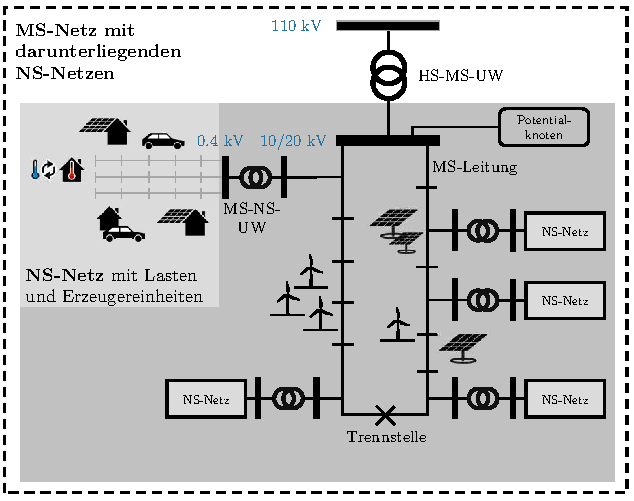
\includegraphics[width=\textwidth]{Bilder/scope_power_flow_kh_cropped}
    \caption[Umfang der Lastflussanalyse mit eDisGo]{Umfang der Lastflussanalyse mit eDisGo \cite{Schachler}}\label{fig:scope}
\end{figure}


\paragraph{Ermittlung des Abregelungsbedarfs für die Auflösung von Netzüberlastungen:}

Die Ermittlung des Abregelungsbedarfs für die Auflösung von Netzüberlastungen erfolgt in einem iterativen Prozess.
Vorerst werden etwaige Netzprobleme und die entsprechenden Zeitschritten in denen die Netzprobleme auftreten mit Hilfe der zuvor beschriebenen Lastflussanalyse ermittelt.
Anschließend wird die Last bzw. die Einspeisung in Schritten von \SI{10}{\percent} innerhalb der ermittelten Zeitschritte gekürzt.
Die beiden Schritte werden so lange wiederholt bis keine Netzprobleme mehr auftreten.\medskip

Die Ermittlung des Abregelungsbedarfs erfolgt für zwei Wochen des Jahres.
Dies ist nötig, um die Rechenzeit innerhalb eines akzeptablen Maßes zu halten.
Hierbei werden die Wochen untersucht, die im Netzgebiet die minimale und maximale durchschnittliche Residuallast aufweisen.
Auf diese Weise sollen möglichst extreme Belastungssituationen abgedeckt werden. \medskip

Bei der Lösung der Netzprobleme werden vorerst Überlastungen gelöst und erst anschließend Spannungsprobleme.
Weiterhin werden Probleme in der \gls{NS}-Ebene gelöst, bevor Probleme in der \gls{MS}-\gls{NS}-Umspannebene und abschließend in der \gls{MS}-Ebene gelöst werden.
Durch die Lösung von Netzproblemen auf tieferen Spannungsebenen können unter Umständen bereits Netzprobleme in darüber liegenden Spannungsebenen gelöst oder entspannst werden.
Weiterhin werden Netzprobleme innerhalb der \gls{NS}- bzw. \gls{MS}-Ebene anhand ihrer Entfernung zur übergeordneten Umspannebene priorisiert.
So kann auch hier die Lösung von weiter entfernten Netzproblemen bereits vorgeschaltete Netzprobleme auflösen oder entspannen.
Für jeden Zeitschritt, in dem Überlastungs- oder Spannungsprobleme an einem Netzknoten auftreten, wird geprüft, ob die Netzprobleme durch hohe Nachfrage oder hohe Einspeisung entstehen.
Anhand dieser Information wird entscheiden, ob Last oder Einspeisung abgeregelt werden soll.\medskip

Aufgrund der hohen Anzahl an \glspl{EPKW}, \glspl{WP} und erneuerbaren Erzeugereinheiten kommt es in einigen Fällen dazu, dass die Lastflussanalyse nicht konvergiert.
In diesen Fällen wird ebenfalls eine Abregelung in den entsprechenden Zeitschritten unternommen.
In diesen Fällen lässt sich dieser Abregelungsbedarf keiner der Netzebenen zuordnen.
Die gesamte notwendige Abregelung für das \gls{MS}-Netz ergibt sich aus der Summierung aller nötigen Abregelungen von Last und Erzeugung am \gls{MS}-Netzanschlusspunkt.
In \autoref{fig:scope_curtailment} findet sich eine Veranschaulichung des Vorgehens.

\begin{figure}[H]
    \centering
    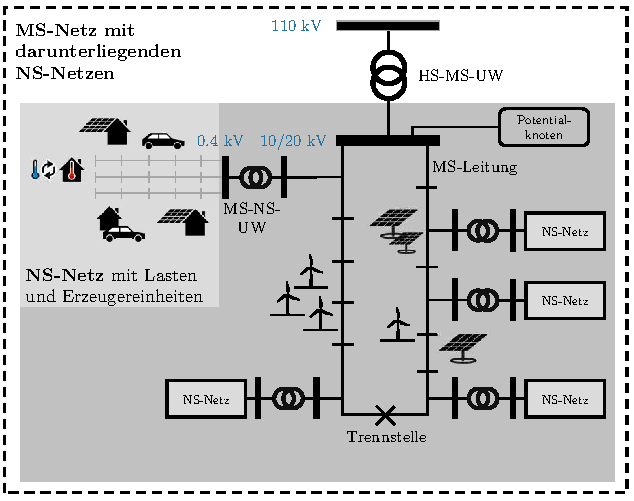
\includegraphics[width=\textwidth]{Bilder/scope_power_flow_kh_cropped}
    \caption[Umfang der Ermittlung des Abregelungsbedarfs für die Auflösung von Netzüberlastungen nach der initialen Überwindung von etwaigen Konvergenzproblemen]{Umfang der Ermittlung des Abregelungsbedarfs für die Auflösung von Netzüberlastungen nach der initialen Überwindung von etwaigen Konvergenzproblemen \cite{Schachler}}\label{fig:scope_curtailment}
\end{figure}

